\documentclass[11pt,twoside,space]{article}
\usepackage{CMC}
\title{第九届中国大学生数学竞赛预赛试卷}
\author{14 金融工程--零蛋大}
\date{2017年10月28日}
\type{数学类}
\examtime{150}
%\watermark{48}{11}{机密}
\begin{document}%\zihao{5}
\maketitle
\begin{center}
\zihao{-4}
\begin{tabular}{|m{3em}<{\centering}|*{7}{m{3.5em}<{\centering}|}}
\hline
题~号 & 一 & 二 & 三  & 四 & 五 & 六  &总~~分 \\
\hline
满~分 & 15 & 15 & 15  & 20 & 15 & 20  &\raisebox{0.38em}{100}\rule{0pt}{8mm}\\
\hline
得~分 &    &    &     &    &    &     &\rule{0pt}{8mm}\\
\hline		
\end{tabular}\vspace*{0.6em}		
$\begin{aligned}
\mbox{注意:}
&1.\,\mbox{所有答题都须写在试卷密封线右边,写在其他纸上一律无效}.\hspace{12.0cm}\\
&2.\,\mbox{密封线左边请勿答题,密封线外不得有姓名及相关标记}.\\
&3.\,\mbox{如答题空白不够,可写在当页背面,并标明题号}.\\[-2mm]
\end{aligned}$A	
\end{center}
\setlength{\marginparsep}{-0.8cm}
%%==================================================================
%%—————————————————————————————正文开始———————————————————————————————
%%==================================================================
%%==================================================================
%%—————————————————————————————正文开始———————————————————————————————
%%==================================================================	

\vspace*{2.5em}
\dati{}{(本题15分)\;\;%\\[2mm]
在空间直角坐标系中,设单叶双曲面 $\Gamma$ 的方程为 $x^2+y^2-z^2=1$,设 $P$ 为空间的平面, 它交 $\Gamma$ 于一抛物线 $C$. 求该平面的法线与 $z$- 轴的夹角.\\} 


\newpage
\dati{}{(本题15分)\;\;
设 $\{a_n\}$ 是递增数列, $a_1>1$. 求证: 级数 $\textstyle\sum\limits_{n=1}^{\infty}\frac{a_{n+1}-a_n}{a_n\ln a_{n+1}}$ 收敛的充分必要条件是 $\{a_n\}$ 有界, 又问级数通项分母中的 $a_n$ 能否换成 $a_{n+1}$?}


\newpage
\dati{}{(本题15分)\;\;
设 $\Gamma=\{W_1,W_2,\cdots,W_r\}$ 为 $r$ 个各不相同的可逆 $n$ 阶复方阵构成的集合. 若该集合关于矩阵乘法封闭(即, $\forall\,M,N\in\Gamma$, 有 $MN\in\Gamma$), 证明:  $\textstyle\sum\limits_{i=1}^{r}W_i=0$
当且仅当 $\textstyle\sum\limits_{i=1}^{r}\text{tr}(W_i)=0$, 其中 $\text{tr}(W_i)$ 表示 $W_i$ 的迹}


\newpage
\dati{}{(本题20分)\;\;
给定非零实数 $a$ 及实 $n$ 阶反对称矩阵 $A$ (即, $A$ 的转置 $A^T$ 等于 $-A$), 记矩阵有序对集合 $T$ 为\[T=\{(X,Y)|X\in\mathbb{R}^{n\times n},Y\in\mathbb{R}^{n\times n},XY=aI+A\},\]}\\[3ex]
其中 $I$ 为 $n$ 阶单位阵, $\mathbb{R}^{n\times n}$ 为所有实 $n$ 阶方阵构成的集合. 证明: 任取 $T$ 中两元: $(X,Y)$ 和 $(M,N)$ 必有 $XN+Y^TM^T\neq0$

\newpage
\dati{}{(本题15分)\;\;
设 $f(x)=\arctan x$, $A$ 为常数. 若
\[B=\lim_{n\to\infty}\bigg(\sum_{k=1}^{n}f\Big(\frac{k}{n}\Big)-An\bigg)\]}\\
存在, 求 $A,B$  



\newpage
\dati{}{(本题20分)\;\;
设 $f(x)=1-x^2+x^3\quad(x\in[0,1])$,\\
计算以下极限并说明理由\[\lim_{n\to\infty}\frac{\scaleobj{0.8}{\displaystyle\int_0^1}f^n(x)\ln(x+2)\dif x}{\scaleobj{0.8}{\displaystyle\int_0^1}f^n(x)\dif x}\]}











%%%%%%%%%%%%%%%%%%%%%%%%%%%%%%%%%%%%%%%%%%%%%%%%%%%%%%%%%%%%%%%%%%%%%
%------------------------------------结束--------------------------------------
%%%%%%%%%%%%%%%%%%%%%%%%%%%%%%%%%%%%%%%%%%%%%%%%%%%%%%%%%%%%%%%%%%%%%
\clearpage
\end{document}




%  合并为一面双页
%  先保存再编译
%  1-6 是从第一页到第六页
\documentclass{article}
\usepackage{pdfpages}
\usepackage[paperwidth=40cm,paperheight=27.5cm]{geometry}
\begin{document}
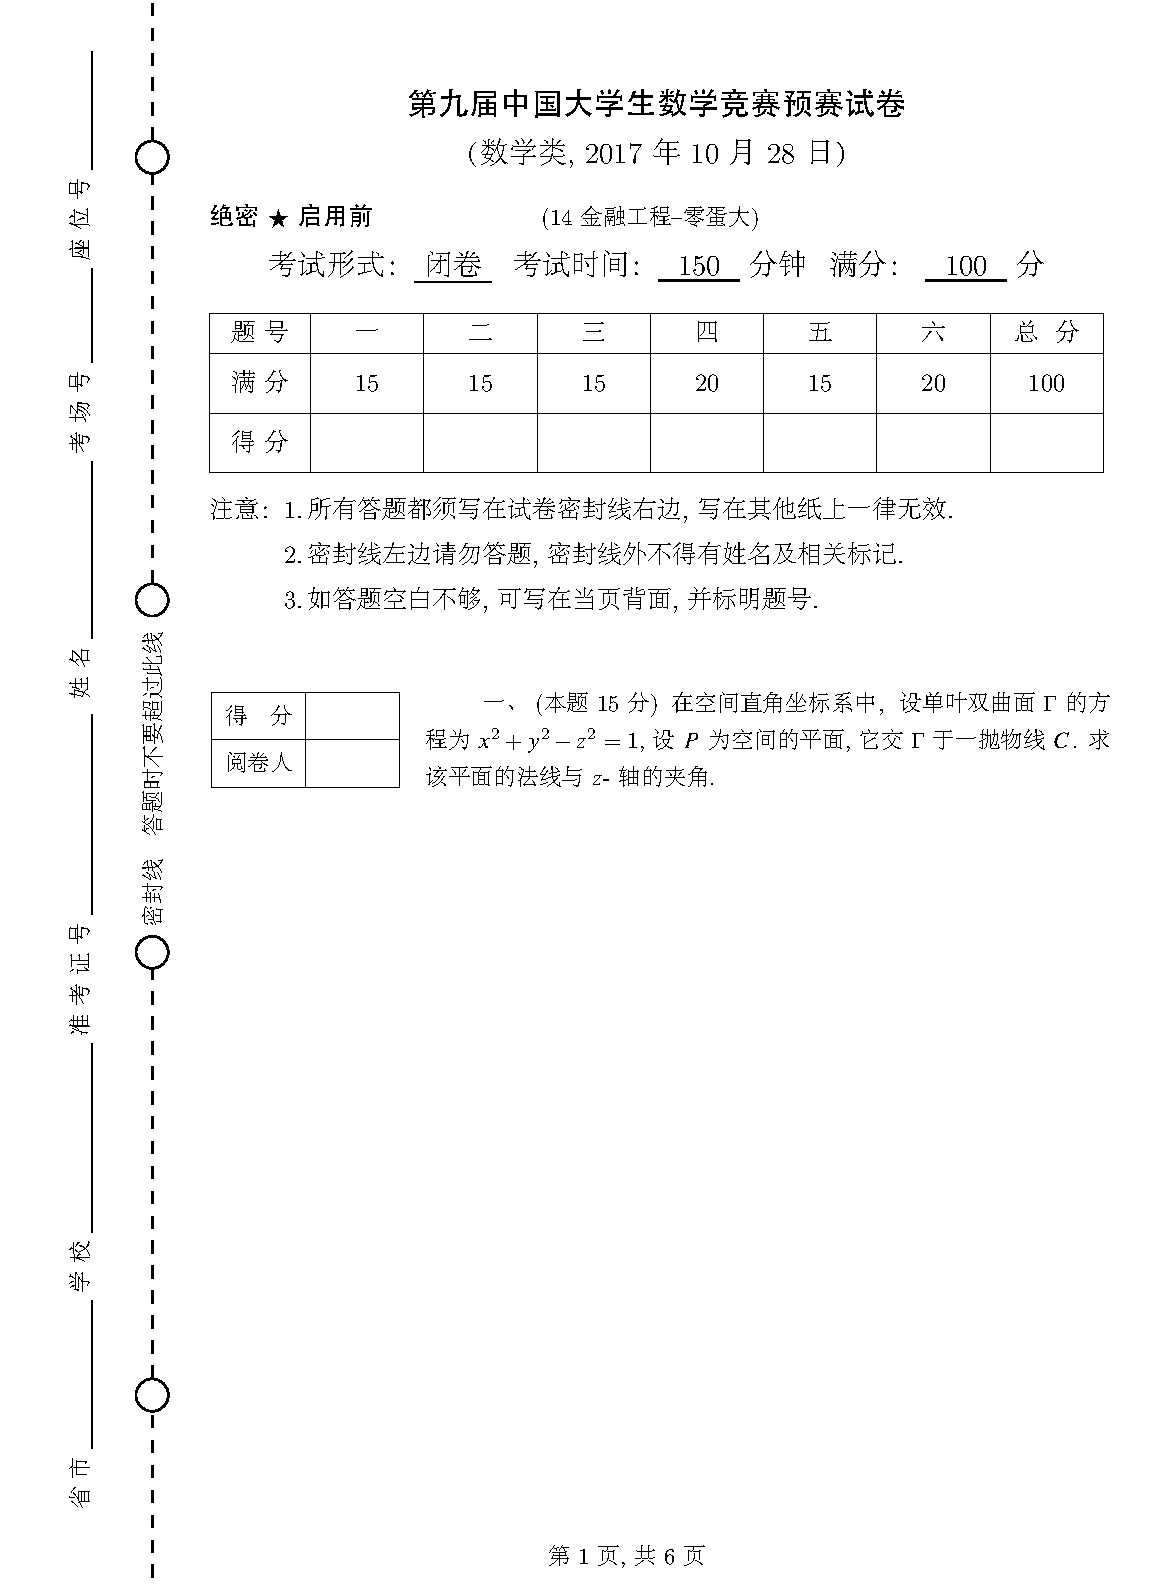
\includepdf[pages=1-6,nup=2x1,scale=1,offset=3mm 0mm,column,delta=-10 -0mm]{17mathSJ.pdf}	
\end{document}

